\documentclass[12pt, oneside, a4paper, chapter=TITLE,section=TITLE]{abntex2}

\usepackage{abntex2-ifrj} % pacote com customizações da classe abntex2 para uso no IFRJ-CVR

%Carregando alguns pacotes extras
\usepackage{float}
\usepackage{scalefnt}
\usepackage{supertabular,booktabs}
\usepackage{multirow}
\usepackage{graphicx}

% ---
% Informações de dados para CAPA e FOLHA DE ROSTO
% ---
\titulo{Totem de Autoatendimento para Restaurantes de Cidades Pequenas: Relatório Final}
\tipotrabalho{Relatório Técnico para Engenharia de Software}
\autor{Alunos: Gabriel Muzel e Mateus Iuri \\ Profa. Dra. Suéllen Martinelli }

\local{Capão Bonito}
\data{\today}
\programa{Tecnologia em Sistemas Inteligentes}
% Preâmbulo
\preambulo{\imprimirtipotrabalho\, desenvolvido pelos alunos Gabriel Muzel e Mateus Iuri como parte dos critérios de avaliação da disciplina ministrada pela Profa. Dra. Suéllen Martinelli. Este documento fecha o ciclo do projeto com o protótipo de média fidelidade, o plano e o instrumento de avaliação, a análise dos dados coletados e os eventos de encerramento do SCRUM.
}

% --------------------------------
\makeindex % compila o índice remissivo (opcional)
% --------------------------------

% --------------------------------
% Início do documento
% --------------------------------
\begin{document}

% Retira espaço extra obsoleto entre as frases.
\frenchspacing

% --------------------------------
% ELEMENTOS PRÉ-TEXTUAIS
% --------------------------------
\pretextual
% ---
\imprimircapa % Capa
\imprimirfolhaderosto % Folha de rosto
% ---

% ---
% lista de ilustrações
\pdfbookmark[0]{\listfigurename}{lof} \listoffigures*
\cleardoublepage
% ---

% ---
% lista de tabelas
\pdfbookmark[0]{\listtablename}{lot}\listoftables*
\cleardoublepage
% ---

% ---
% inserir lista de quadros
\pdfbookmark[0]{\listofquadrosname}{loq} \listofquadros*
\cleardoublepage
% ---

% ---
% inserir lista de abreviaturas e siglas (opcional)
\begin{siglas}
  \item[ABNT] Associação Brasileira de Normas Técnicas
  \item[CSV] \textit{Comma-Separated Values}
  \item[LF] Baixa Fidelidade
    \item[PO] Product Owner
  \item[SM] Scrum Master
  \item[TCLE] Termo de Consentimento Livre e Esclarecido
  \item[UC] Caso de Uso
  \item[US] História de Usuário
  \item[WIP] Work In Progress
\end{siglas}
% ---

% ---
% inserir lista de símbolos
% ---
\begin{simbolos}
  \item[$N$] Número de participantes da avaliação
\end{simbolos}
% ---

% ---
% sumario
\pdfbookmark[0]{\contentsname}{toc}
\tableofcontents*
% ---

% --------------------------------
% ELEMENTOS TEXTUAIS
\textual
% --------------------------------

\chapter{Introdução}

Este relatório final documenta a conclusão do projeto ``Totem de Autoatendimento para Restaurantes de Cidades Pequenas'', desenvolvido na disciplina de Engenharia de Software da FATEC Capão Bonito por Gabriel Muzel e Mateus Iuri, sob orientação da Profa. Dra. Suéllen Martinelli.

A Parcial 1 registrou a descoberta, a pesquisa com 13 clientes, a Matriz CSD, as sete Histórias de Usuário e o planejamento da Sprint 1. A Parcial 2 documentou a prototipação de baixa fidelidade, os diagramas de caso de uso, a matriz de feedback e os eventos de Sprint Review e Retrospectiva da primeira sprint. Esta entrega fecha o ciclo com o protótipo de média fidelidade usado na avaliação, o plano e o instrumento aplicados, os dados anonimizados, as análises quantitativa e qualitativa e o registro das mudanças de produto e processo.

A US07 (Suporte ao Atendente) foi registrada na Parcial 1, mas ficou fora do escopo avaliado nesta entrega: não há aplicativo de atendente, e a acessibilidade foi tratada pelo modo fácil do próprio totem.

\chapter{Características do Projeto}

O produto avaliado é um totem de autoatendimento com tela sensível ao toque para restaurantes de cidades pequenas. As funcionalidades avaliadas abrangem US01 a US06: visualizar cardápio com fotos, adicionar itens e quantidade, personalizar pedido, pagar com cartão ou PIX, emitir senha de retirada e oferecer modo de acessibilidade.

A versão final do protótipo é de média fidelidade: mantém a navegação e os controles do produto, com cores, hierarquia visual e estados de sucesso, mas sem implementação de backend. Foi usada como estímulo único na avaliação com usuários.

\section{Problema e Objetivo}

\textbf{Problema:} antes da implementação definitiva, é necessário verificar se o fluxo de pedido é compreensível, rápido e acessível, especialmente para clientes com pouca familiaridade tecnológica.

\textbf{Objetivo geral:} avaliar a usabilidade do protótipo de média fidelidade e consolidar as decisões finais de produto e processo.

\begin{itemize}
    \item Aplicar um roteiro de execução com tarefas vinculadas às User Stories.
    \item Coletar dados anonimizados de 16 participantes.
    \item Gerar análises quantitativa e qualitativa, com gráficos em formatos distintos.
    \item Registrar Sprint Review, Retrospectiva e as alterações no Kanban e no \textit{Product Backlog}.
\end{itemize}

\section{Metodologia Utilizada: SCRUM}

O SCRUM organiza o trabalho em papéis, artefatos e eventos \cite{schwaber2017scrum}. A avaliação final corresponde ao incremento apresentado na Sprint Review e sua retrospectiva alimenta o \textit{Product Backlog}. A Engenharia de Requisitos sustenta a redação das Histórias de Usuário e dos critérios de aceitação \cite{wazlawick2019engenharia}.

\chapter{Entrega Final}

\section{Protótipo de Média Fidelidade usado na avaliação}

O protótipo final cobre todas as User Stories do escopo avaliado (US01 a US06) e foi disponibilizado como modelo dinâmico no Figma: \url{https://www.figma.com/make/K5XkfIlE4NsOd0QDdhzcSx/Restaurant-Kiosk-App-Design?t=oOAOxDcetEklvcdI-20&fullscreen=1}. As telas incluem cardápio por categorias, modo fácil, carrinho, personalização, pagamento integrado e senha de retirada.

\section{Plano de Avaliação}

O plano de avaliação foi organizado em seis etapas: (1) recrutamento de voluntários; (2) aplicação do TCLE; (3) explicação do objetivo e do protótipo; (4) execução das tarefas; (5) resposta ao instrumento; (6) encerramento e agradecimento.

\begin{table}[ht]
\centering
\caption{Roteiro de execução da avaliação.}
\resizebox{\textwidth}{!}{%
\begin{tabular}{@{}p{1.2cm}p{5cm}p{6cm}@{}}
\toprule
\textbf{Tarefa} & \textbf{Ação do participante} & \textbf{US relacionada} \\ \midrule
T1 & Abrir o cardápio, localizar o X-Burger e verificar foto e preço & US01 \\
T2 & Adicionar um X-Burger e dois refrigerantes, depois aumentar a quantidade & US02 \\
T3 & Personalizar o X-Burger: remover tomate e adicionar bacon & US03 \\
T4 & Finalizar o pedido e escolher PIX ou cartão & US04 \\
T5 & Identificar a senha mostrada ao final do pagamento & US05 \\
T6 & Ativar o modo de acessibilidade e ler o texto ampliado & US06 \\ \bottomrule
\end{tabular}%
}
\end{table}

As métricas observadas foram: conclusão de cada tarefa (sim/não), tempo total de execução em segundos, satisfação de 1 a 5 e comentário livre ao final.

\section{Instrumento de Avaliação aplicado}

O instrumento foi um formulário online anônimo, com consentimento inicial, seis blocos de tarefa, escala de satisfação e perguntas abertas. Link de acesso: \url{https://forms.gle/ESZt6PGCqa6aX3nm9}.

\section{Dados anonimizados das avaliações}

Os dados anonimizados foram obtidos no teste do protótipo. A Tabela~\ref{tab:modelo_avaliacao} apresenta o conjunto correspondente aos participantes P1 a P16.

\begin{table}[ht]
\centering
\caption{Dados anonimizados das avaliações.}
\label{tab:modelo_avaliacao}
\resizebox{\textwidth}{!}{%
\begin{tabular}{@{}p{1.3cm}p{1.1cm}p{1.1cm}p{1.1cm}p{1.1cm}p{1.1cm}p{1.1cm}p{1.5cm}p{1.3cm}p{4.5cm}@{}}
\toprule
\textbf{Part.} & \textbf{T1} & \textbf{T2} & \textbf{T3} & \textbf{T4} & \textbf{T5} & \textbf{T6} & \textbf{Tempo (s)} & \textbf{Satisfação} & \textbf{Comentário} \\ \midrule
P1 & Sim & Sim & Sim & Sim & Sim & Sim & 285 & 5 & Sou usuária de apps e achei rapidí... \\
P2 & Com dificuldade & Não & Não & Com dificuldade & Sim & Com dificuldade & 715 & 3 & Não sou de tecnologia, mas sinto f... \\
P3 & Sim & Sim & Sim & Sim & Sim & Sim & 338 & 4 & Ótimo para o dia a dia, mas ainda ... \\
P4 & Sim & Sim & Sim & Sim & Não & Sim & 315 & 5 & muito bom memo, so q a senha num a... \\
P5 & Sim & Sim & Sim & Sim & Sim & Sim & 292 & 5 & Como como sempre aqui, quero só ag... \\
P6 & Com dificuldade & Sim & Não & Com dificuldade & Sim & Não & 570 & 3 & Achei bonito, mas tenho medo de er... \\
P7 & Sim & Sim & Sim & Sim & Sim & Sim & 241 & 5 & Achei intuitivo demais. Até meu av... \\
P8 & Sim & Sim & Sim & Não & Sim & Não & 475 & 3 & Sou cético com totem. Se o pagamen... \\
P9 & Sim & Com dificuldade & Sim & Sim & Sim & Com dificuldade & 373 & 4 & Gostei, mas preciso testar com min... \\
P10 & Sim & Sim & Sim & Sim & Sim & Sim & 169 & 5 & Melhor que fila. Só falta um modo ... \\
P11 & Com dificuldade & Com dificuldade & Não & Com dificuldade & Sim & Com dificuldade & 690 & 4 & Nunca usei totem, mas com as letra... \\
P12 & Sim & Sim & Sim & Sim & Sim & Sim & 298 & 5 & Como cuido da alimentação, a perso... \\
P13 & Sim & Não & Não & Sim & Sim & Não & 440 & 3 & Sou daqueles que quer só o essencial: menos botão, mais direto \\
P14 & Sim & Sim & Sim & Sim & Sim & Sim & 273 & 5 & Como dono de negócio, vejo valor: ... \\
P15 & Sim & Sim & Sim & Sim & Não & Sim & 315 & 4 & Pego pedido rapidinho. Quando a se... \\
P16 & Sim & Sim & Sim & Sim & Sim & Sim & 221 & 5 & Adorei! Já indiquei para meus amig... \\ \bottomrule
\end{tabular}%
}
\end{table}

\section{Análise quantitativa dos dados}

Os seis gráficos abaixo derivam do conjunto registrado em \texttt{dados/formulario2.csv}. Há seis gráficos quantitativos, em barras verticais, barras horizontais, pizza, rosca, \textit{boxplot} e linha, e dois gráficos qualitativos. Para fins de taxa de conclusão, as respostas ``Sim'' e ``Sim, com dificuldade'' foram somadas. A satisfação teve mediana 4,5, com 75\% das notas entre 4 e 5. A T1 foi concluída por 16 participantes e a T4 por 15; a T3 teve o menor índice (12 de 16), concentrando as dificuldades na personalização do pedido.

\begin{figure}[ht]
\centering
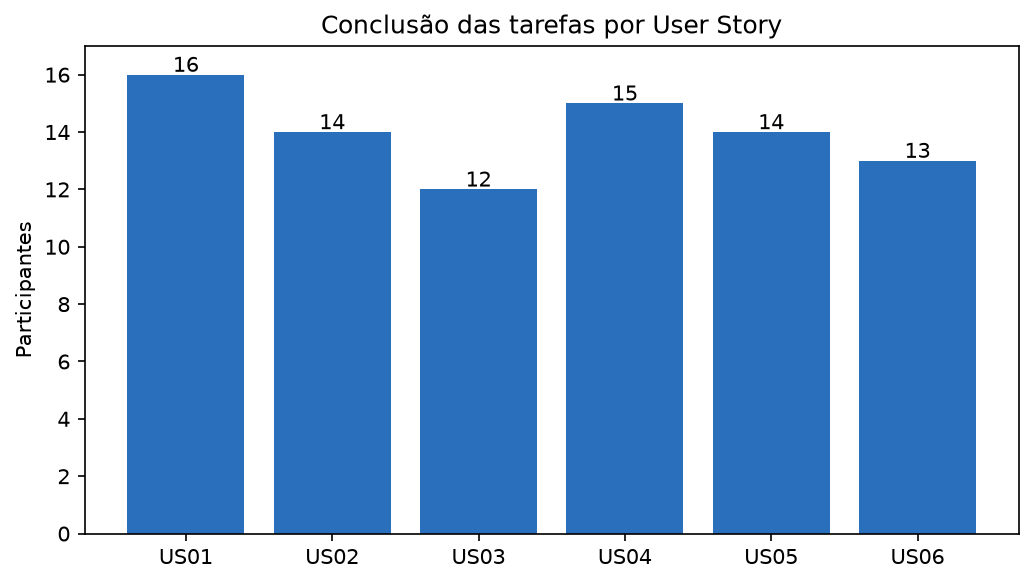
\includegraphics[width=0.8\textwidth]{graficos/01_conclusao_us.png}
\caption{Conclusão das tarefas por User Story.}
\end{figure}

\begin{figure}[ht]
\centering
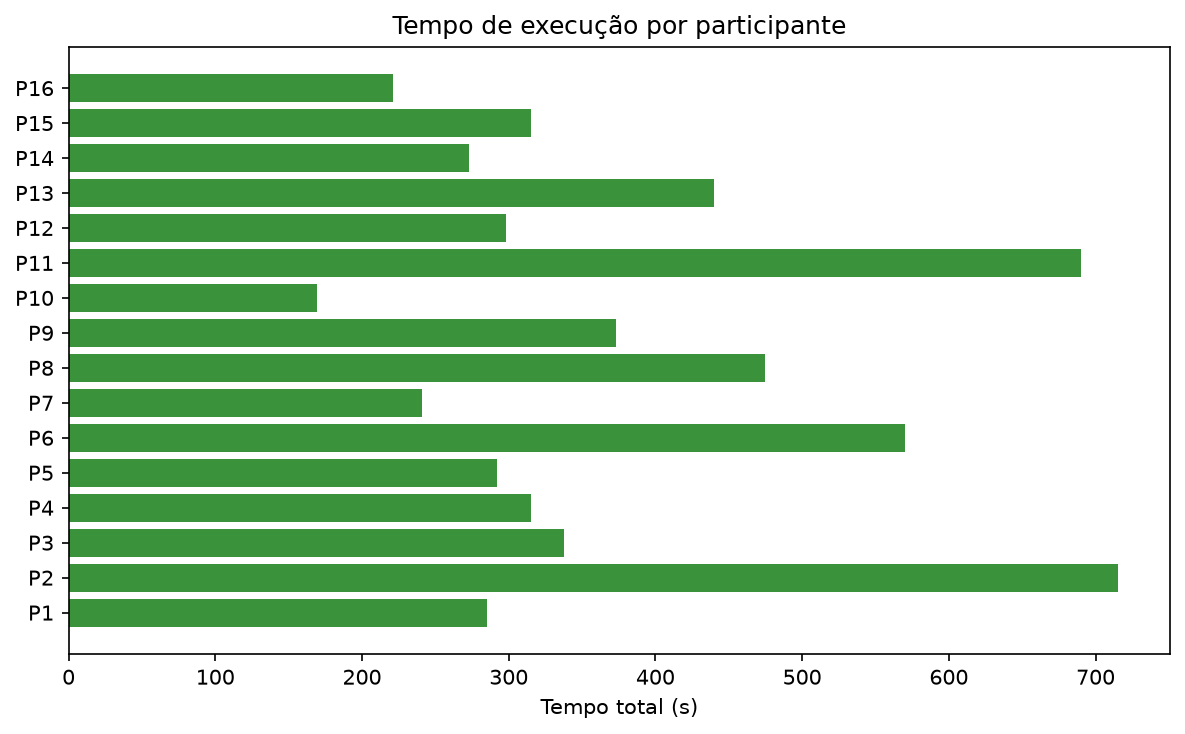
\includegraphics[width=0.8\textwidth]{graficos/02_tempo_participante.png}
\caption{Tempo de execução por participante.}
\end{figure}

\begin{figure}[ht]
\centering
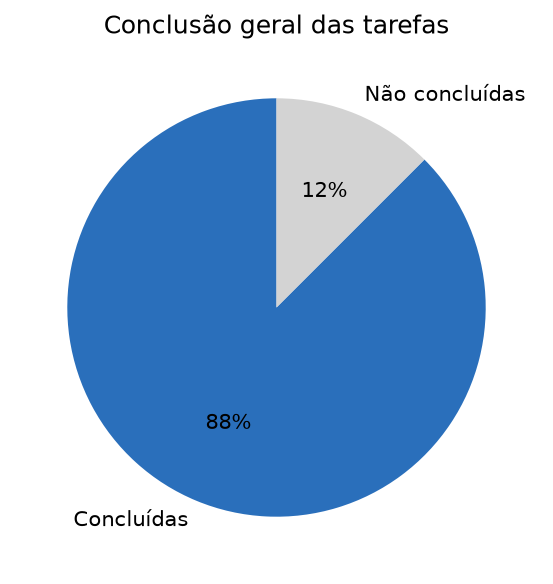
\includegraphics[width=0.6\textwidth]{graficos/03_conclusao_pizza.png}
\caption{Conclusão geral das tarefas.}
\end{figure}

\begin{figure}[ht]
\centering
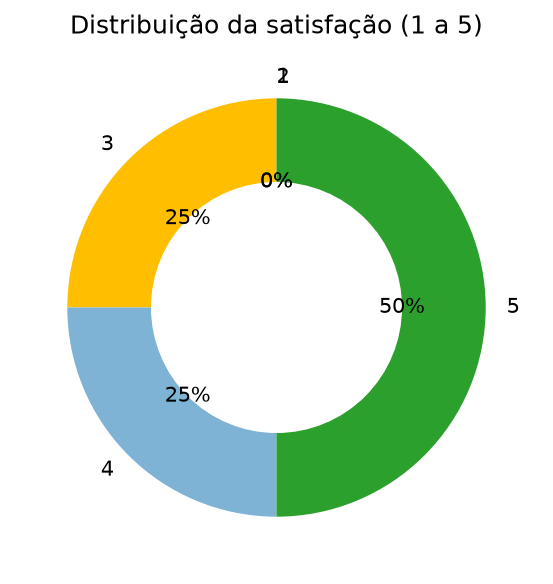
\includegraphics[width=0.6\textwidth]{graficos/04_satisfacao_donut.png}
\caption{Distribuição da satisfação (1 a 5).}
\end{figure}

\begin{figure}[ht]
\centering
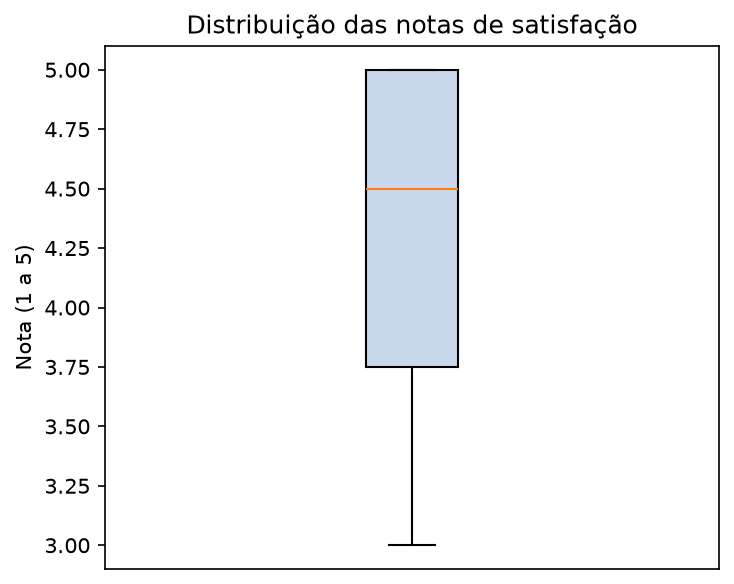
\includegraphics[width=0.6\textwidth]{graficos/05_satisfacao_boxplot.png}
\caption{\textit{Boxplot} das notas de satisfação.}
\end{figure}

\begin{figure}[ht]
\centering
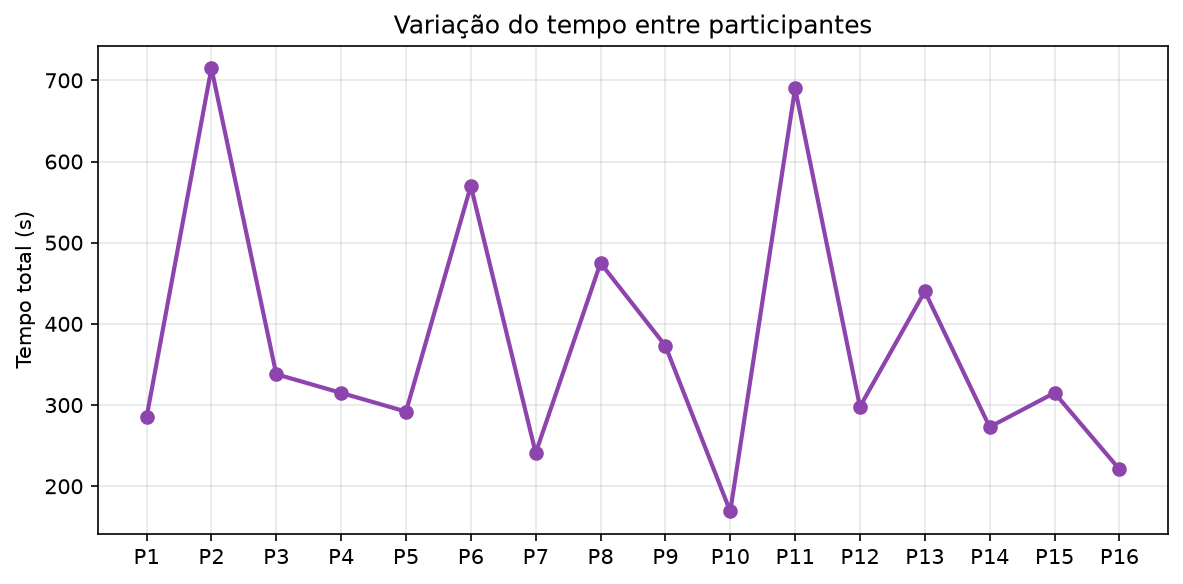
\includegraphics[width=0.8\textwidth]{graficos/06_tempo_linha.png}
\caption{Variação do tempo entre participantes.}
\end{figure}

\section{Análise qualitativa dos dados}

A matriz de captura de feedback da Parcial 2 serviu de referência. As 16 respostas abertas do formulário final foram codificadas em cinco temas: idosos e acessibilidade (5 menções), design e intuitividade (4), tempo e rapidez (4), pagamento (2) e senha de retirada (2). Os dois gráficos seguintes apresentam essa codificação em formatos distintos.

\begin{figure}[ht]
\centering
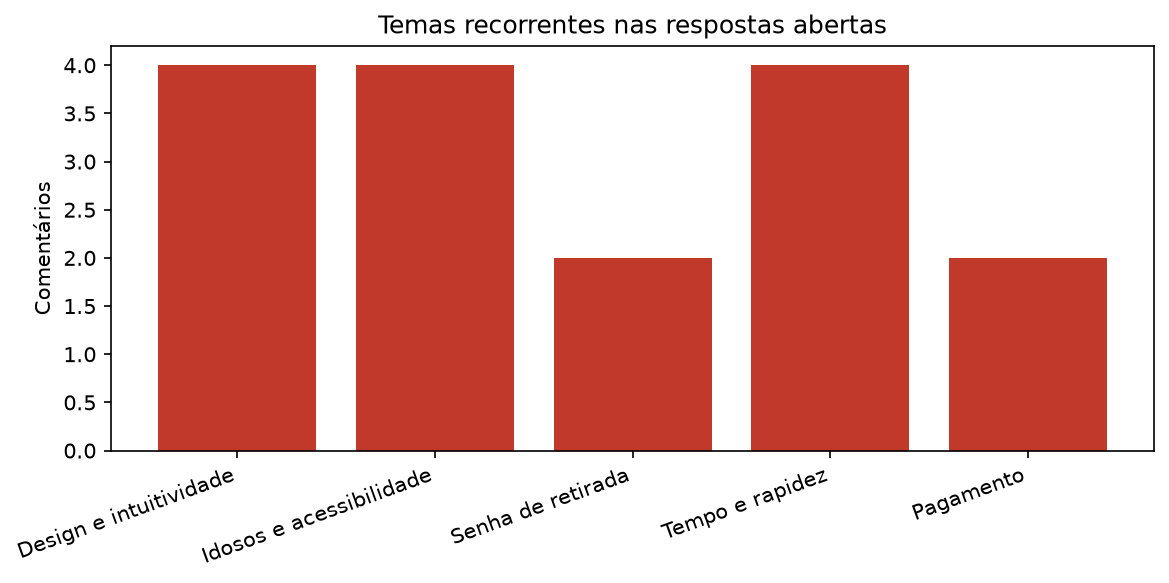
\includegraphics[width=0.8\textwidth]{graficos/07_temas_qualitativos.png}
\caption{Temas recorrentes nas respostas abertas.}
\end{figure}

\begin{figure}[ht]
\centering
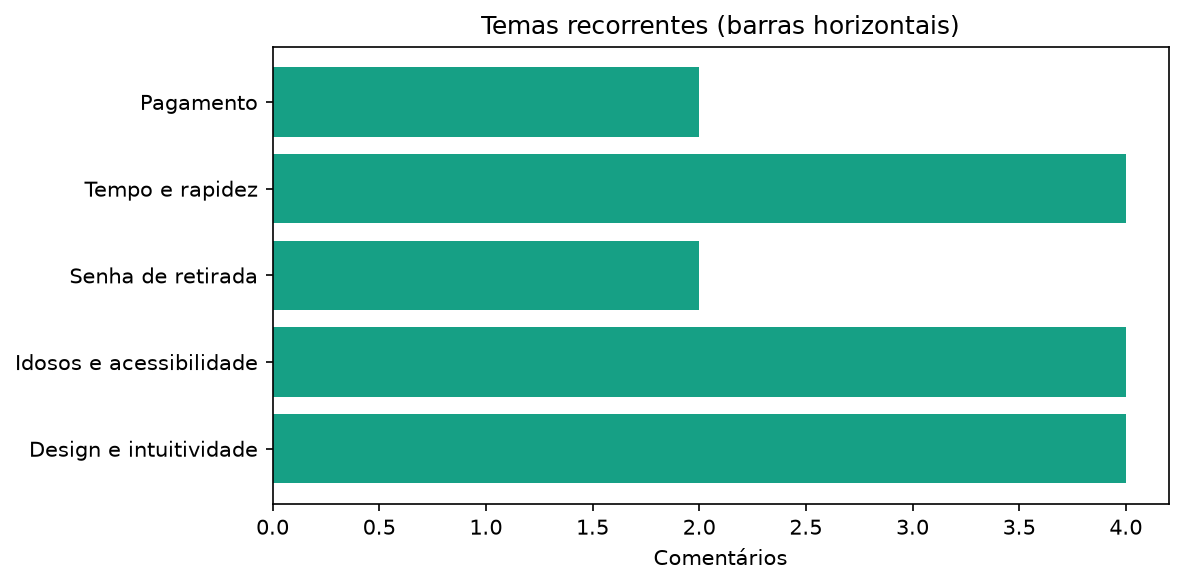
\includegraphics[width=0.8\textwidth]{graficos/08_temas_horizontais.png}
\caption{Temas qualitativos em barras horizontais.}
\end{figure}

\section{Sprint Review, Retrospectiva e alterações de produto}

A Sprint Review e a Retrospectiva da Parcial 2, realizadas em 26/10/2026 com Gabriel Muzel e Mateus Iuri, são retomadas aqui como base para as decisões da entrega final.

Na Sprint Review da Parcial 2, o roteiro de demonstração cobriu os itens 01 e 02 do \textit{Product Backlog}; o item 03 foi demonstrado como protótipo, mas não concluído: visualizar cardápio com fotos, adicionar ao carrinho e personalização de itens. A Tabela~\ref{tab:review_final} retoma esse roteiro e registra o destino das histórias observado no quadro Kanban.

\begin{table}[ht]
\centering
\caption{Roteiro de demonstração e destino das histórias no Kanban.}
\label{tab:review_final}
\resizebox{\textwidth}{!}{%
\begin{tabular}{@{}p{4.2cm}p{4cm}p{5cm}@{}}
\toprule
\textbf{História} & \textbf{Antes (Parcial 2)} & \textbf{Depois} \\ \midrule
US01: Visualizar Cardápio & Sprint Backlog & Done \\
US02: Adicionar Item e Quantidade & Sprint Backlog & Done \\
US03: Personalizar Pedido & Sprint Backlog & Product Backlog, não concluída \\
US04: Realizar Pagamento & Product Backlog & Product Backlog \\ \bottomrule
\end{tabular}%
}
\end{table}

A Retrospectiva apontou como pontos de atenção a consolidação dos dados de avaliação e a reestimativa da US03. Como ação combinada, o time manteve a acessibilidade como item prioritário no \textit{Product Backlog}.

\section{Links de acesso ao projeto}

\begin{table}[ht]
\centering
\caption{Artefatos e links de acesso.}
\resizebox{\textwidth}{!}{%
\begin{tabular}{@{}p{4.2cm}p{10cm}@{}}
\toprule
\textbf{Artefato} & \textbf{Local / link} \\ \midrule
Repositório Git & \url{https://github.com/Fatec-activities-cb/eng-de-software.git} \\
Quadro Kanban (Trello) & \url{https://trello.com/invite/b/6ad94663283aa9fb3397a1d4/ATTI75eb7223eddb3d284cc9695b8728757a2B864393/kanban} \\
Diagrama de caso de uso (Lucidchart) & \href{https://lucid.app/lucidchart/87d422f6-cbc5-4222-96b6-cc3525e06341/edit?invitationId=inv_f1629cb9-e852-4390-acda-172a5c572f27\&page=0_0\#}{Lucidchart (diagrama editável)} \\
Protótipo no Figma & \href{https://www.figma.com/make/K5XkfIlE4NsOd0QDdhzcSx/Restaurant-Kiosk-App-Design?t=oOAOxDcetEklvcdI-20\&fullscreen=1}{Figma (versão final)} \\
Instrumento de avaliação & \url{https://forms.gle/ESZt6PGCqa6aX3nm9} \\
Dados da avaliação & arquivo local \texttt{dados/formulario2.csv} \\ \bottomrule
\end{tabular}%
}
\end{table}

Os relatórios, o CSV, os gráficos e as imagens estão versionados no repositório GitHub.

% ---------------------------------
% ELEMENTOS PÓS-TEXTUAIS
% ---------------------------------
\phantompart
\postextual

% ---------------------------------
% Referências bibliográficas
% ---------------------------------
\bibliography{../documentos/references}

% ---------------------------------
% Glossário
% ---------------------------------

% ---------------------------------
% Apêndices
% ---------------------------------
\begin{apendicesenv}
\partapendices

\chapter{Termo de Consentimento Livre e Esclarecido}

\begin{figure}[!ht]
\setlength{\itemsep}{0pt}
\setlength{\parskip}{0pt}
\centering
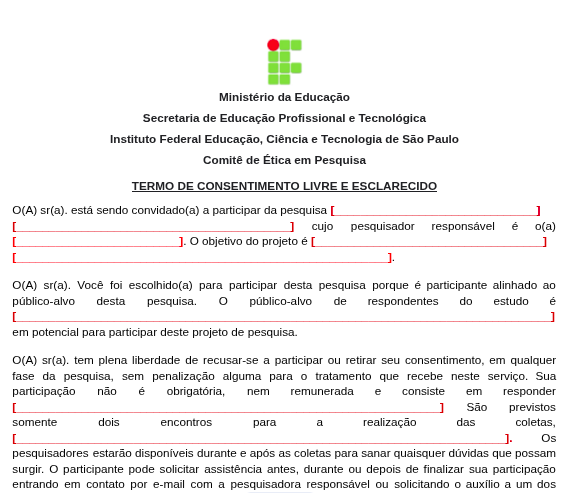
\includegraphics[width=0.7\columnwidth]{imagens/print_TCLE.png}
\caption{Formulário de consentimento apresentado na pesquisa.}
\end{figure}

\end{apendicesenv}

% ----------------------------------------------
% Anexos
% ----------------------------------------------
\begin{anexosenv}
\partanexos

\chapter{Quadro Kanban}

O quadro digital está disponível no link da Tabela de acesso. As imagens \texttt{kanban1.jpeg} e \texttt{kanban2.jpeg}, mantidas em \texttt{documentos/}, registram o antes e o depois da Sprint 1.

\end{anexosenv}

%------------------------------------------------------
% INDICE REMISSIVO
%------------------------------------------------------
\phantompart
\printindex

\end{document}
